

\section{Appendix for Section 2: $L_1$-perturbations}

\label{app.L1}

\setcounter{proposition}{1}



\begin{proposition}
	The following system of LP constraints is equivalent with $\sum_{j\leq k} |x_j-x'_j| \leq \varepsilon$ ($L_1$-perturbation):
	
	\begin{enumerate}
		\item for all {\em input} neuron $j$ (in layer 0), 
		$A_j \geq x_j - x'_j $ and $A_j \geq x'_j - x_j$,
		
		\item $\sum_{j\leq k} A_j \leq \varepsilon$.
	\end{enumerate}
\end{proposition}


\begin{proof}[Proof] First implication: For any solution to the constraint $\sum_{j\leq k} |x_j-x'_j| \leq \varepsilon$, we show that it also satisfies the combined constraints. 
	%Notice that the variables $A_j$ only appear in this group of constraints. So 
	We let $A_j = |x_j-x'_j|$ for each $j$. For each $j$, $A_j = |x_j-x'_j|\geq x_j - x'_j, A_j = |x_j-x'_j|\geq x'_j - x_j$,  and $$\sum_{j\leq k} A_j = \sum_{j\leq k} |x_j-x'_j| \leq\varepsilon.$$
	
	
Reverse implication: Similarly, if $A_j$ satisfies the system of LP constraints, then for any $j$, we have $$A_j \geq \max\{x'_j - x_j, x_j - x'_j\} = |x_j-x'_j|.$$ Hence $$\sum_{j\leq k} |x_j-x'_j| \leq \sum_{j\leq k} A_j\leq\varepsilon.$$
\end{proof}



\section{Appendix for Section 3: Real-Time Certification}

\label{app.realtime}

\begin{proposition}
If "certified robust" is returned over input $I$, 
then for all perturbed input $I'$ with  $|I - I'| \leq \varepsilon$,
the DNN has the same decision on $I$ and on $I'$, i.e. the DNN is robust around $I$. % for perturbation $\varepsilon$.
\end{proposition}

\begin{proof}[Proof] By definition, "certified robust" means that for any $D\neq C$, $b_D = 0$, which means that $\bar{\beta}^{\varepsilon}_{C,D} < x_C - x_D$. 

Then by the definition, for the image $I'$ that $|I - I'|\leq \varepsilon$, we have $(x_C-x_D) - (x'_C-x'_D)\leq \bar{\beta}^{\varepsilon}_{C,D}$. Hence, $x'_C-x'_D\geq (x_C-x_D)-\bar{\beta}^{\varepsilon}_{C,D}> 0$. This argument works for all $D\neq C$, therefore, the output for $I'$ is still $C$.
\end{proof}

We now compare our bound $\beta$ with the bound $\alpha$ considered by Vhagar \cite{vhagar}, for an evaluation purpose only (how narrow is the gap) rather than to verify robustness in real-time. 
Namely, VHAGaR \cite{vhagar} defines $\alpha^{\varepsilon}_{C,D}$, computing the perturbation necessary to switch an image classified as class $C$ into an image classified as class $D$:
\begin{align*}
	\alpha^{\varepsilon}_{C,D} &= \max_{|I-I'| \leq \varepsilon} (x_C-\max_{E\neq C}x_E) &\text{s.t. }  x'_D \geq \max_{E\neq D}x'_E \wedge x_C \geq \max_{E\neq C}x_E 
\end{align*}

Notice that  
$\alpha^{\varepsilon}_{C,D}$ is not symmetrical, while 
$\beta^{\varepsilon}_{C,D}$ is.


\section{Appendix for Section 4: LAE-DNN}
\label{app.lae.folding}

We show that an LAE-DNN can be represented with the same architecture
as the original DNN by absorbing the linear transformation of
LAE-encode and LAE-decode into the first linear layer of the DNN.

Let LAE-encode be represented by a matrix
$\boldsymbol{W}^{\mathrm{enc}}\in\mathbb{R}^{n\times d_0}$ and
LAE-decode by a matrix
$\boldsymbol{W}^{\mathrm{dec}}\in\mathbb{R}^{d_0\times n}$.
Hence, for an input $\boldsymbol{x}\in\mathbb{R}^{d_0}$, the projected
input produced by the LAE is
\[
\boldsymbol{W}^{\mathrm{dec}}
\boldsymbol{W}^{\mathrm{enc}}\boldsymbol{x}.
\]

\noindent\textbf{Proposition.}
\emph{Let $f$ be an $\ell$-layer DNN with weight matrices
	$\boldsymbol{W}^i$ and bias vectors $\vb^i$, as defined in
	Section~\ref{s.notation}. The LAE-DNN can be represented by an
	$\ell$-layer DNN with the same layer dimensions and ReLU activations
	as $f$, by changing only the weight matrix of its first layer.}


\begin{proof}[Proof]
	The pre-activation values of the first layer of the LAE-DNN are
	\begin{align*}
		\boldsymbol{z}_{\mathrm{LAE}}^1
		&=
		\boldsymbol{W}^1
		\left(
		\boldsymbol{W}^{\mathrm{dec}}
		\boldsymbol{W}^{\mathrm{enc}}\boldsymbol{x}
		\right)
		+\vb^1 \\
		&=
		\left(
		\boldsymbol{W}^1
		\boldsymbol{W}^{\mathrm{dec}}
		\boldsymbol{W}^{\mathrm{enc}}
		\right)\boldsymbol{x}
		+\vb^1.
	\end{align*}
	Define
	\[
	\widetilde{\boldsymbol{W}}^1
	=
	\boldsymbol{W}^1
	\boldsymbol{W}^{\mathrm{dec}}
	\boldsymbol{W}^{\mathrm{enc}}.
	\]
	We then have
	\[
	\boldsymbol{z}_{\mathrm{LAE}}^1
	=
	\widetilde{\boldsymbol{W}}^1\boldsymbol{x}
	+\vb^1.
	\]
	Thus, the LAE transformation is absorbed into the weight matrix of
	the first layer, while its bias vector remains unchanged.
	
	All subsequent weight matrices and bias vectors remain unchanged.
	Therefore, all subsequent pre-activation and post-activation values,
	and in particular the output $\boldsymbol{z}^{\ell}$, are identical.
	
	Finally,
	\[
	\widetilde{\boldsymbol{W}}^1
	\in\mathbb{R}^{d_1\times d_0},
	\]
	which is the same dimension as $\boldsymbol{W}^1$. Hence, this
	transformation changes neither the number of layers nor their
	dimensions, and the resulting DNN computes exactly the same function
	as the LAE-DNN.
\end{proof}


%\section{Appendix for Section 5: LAE-DNN}
%
%
%
%Let us precise LAE-encode and LAE-decode properties.
%LAE-encode defines $n$ independent vectors of dimension $1\times dim$.
%We can complete it in a basis $B'$ of size $dim$.
%There exists a basis transformation from the natural basis of dimension $dim$ 
%to $B'$. As explained, the optimal choice for LAE-encode is to mimic the basis transformation, dropping all the coefficients not corresponding to the first $n$ coefficients. Hence, LAE-decode(LAE-encode) is a projection on these $n$ independent vectors, no matter how LAE-encode, LAE-decode are constructed: the only choice for LAE is the choice of the $n$ independent vectors to project on.
%
%\begin{proposition}
%	\label{Prop3}
%	For all DNN and all latent space dimension $n$, $\beta^\varepsilon_{C,D}(\text{LAE-DNN}) \leq \beta^{\varepsilon}_{C,D}(\text{DNN})$.
%\end{proposition}
%
%\begin{proof}[Proof] 
%	Let $(I,I')$ be a pair of image and its perturbation maximizing $\beta^\varepsilon_{C,D}(\text{LAE-DNN})$. Let $J$ be the projected input 
%	$J=$LAE-decode(LAE-encode($I$)) from $I$.
%	We have $J=$LAE-decode(LAE-encode($J$)) as a projection is invariant.
%	The same is true for $J'=$LAE-decode(LAE-encode($J'$)) the projected input
%	from $I'$. 
%	Hence $J,J'$ also maximizes $\beta^\varepsilon_{C,D}(\text{LAE-DNN})$.
%	
%    $J,J'$ are valid inputs for DNN as well, with the same $x_C-x_D+x'_D-x'_C$
%	as $\beta^\varepsilon_{C,D}(\text{LAE-DNN})$. Hence, $\beta^\varepsilon_{C,D}(\text{LAE-DNN}) \leq \beta^{\varepsilon}_{C,D}(\text{DNN})$.
%\end{proof}
%
%Some may see Out of Distribution (OOD) detection as an alternative to (L)AE-DNN. 
%There is a key difference: in OOD detection, the main problem is OOD inputs leading to output of DNN very similar to ID inputs. In OOD detection, these are dangerous inputs, not easy to detect and filter out. 
%In our case, these inputs are perfectly harmless, as 
%they do not increase the bound $\bar{\beta}^{\varepsilon}_{C,D}$. 
%What we need to filter out are OOD inputs leading to outputs of the DNN that are far away from ID outputs, which are the ones creating large bounds $\bar{\beta}^{\varepsilon}_{C,D}$.
%
%Reciprocally, (L)AE-DNN does not overcome the issue considered by OOD detection either: (L)EA-DNN could still provide a label (with high confidence) that does not correspond with the (OOD) input. LAE-DNN focuses on ensuring that the answer given will be robust, i.e., small changes in the input will not modify the output too much, but prediction on the image and its perturbation could be equally misleading. The bottom line is that OOD detection is orthogonal to the focus of (L)AE-DNN.


\section{Appendix for Section 5: {\em Diff} and {\em 1b} MILP models}

We first prove that the {\em Diff} model encodes exactly $\hat{y}$.

\begin{proposition}
	\label{Prop4}
	Assuming $y_j \in [-\gamma_j, \gamma_j]$ and $x'_j,y_j+x'_j \in [\alpha_j,\beta_j]$, we have that $\hat{y}_j = \ReLU(x_j=y_j + x'_j) - \ReLU(x'_j)$ is the solution of the MILP program:
	\begin{align*}
		& \begin{aligned}
			y_j + x'_j &\leq a\beta_j        &
			y_j &+ x'_j \geq (1-a)\alpha_j \\
			x'_j       &\leq a'\beta_j       & 
			x'_j       &\geq (1-a')\alpha_j \\
			\hat{y}_j  &\leq a\gamma_j       &
			\hat{y}_j  &\geq -a'\gamma_j \\
			\hat{y}_j  &\leq y_j + x'_j - (1-a)\alpha_j &
			\hat{y}_j  &\geq y_j + x'_j - a'\beta_j \\
			\hat{y}_j  &\leq -x'_j + a\beta_j &
			\hat{y}_j  &\geq -x'_j + (1-a')\alpha_j \\
			\hat{y}_j  &\leq y_j + (1-a)\gamma_j  &
			\hat{y}_j  &\geq y_j - (1-a')\gamma_j
		\end{aligned}
	\end{align*} 
	where $a,a' \in \{0,1\}$ are binary variables, 
	and $a'$ is shared with the classical MILP
	encoding for $\hat{x}'_j=\ReLU(x'_j)$.
\end{proposition}

\begin{proof}[Proof]
	First, we list the inequalities: \begin{align*}
		& \begin{aligned}
			y_j + x'_j &\leq a\beta_j        &
			y_j &+ x'_j \geq (1-a)\alpha_j \\
			x'_j       &\leq a'\beta_j       & 
			x'_j       &\geq (1-a')\alpha_j \\
			\hat{y}_j  &\leq a\gamma_j       &
			\hat{y}_j  &\geq -a'\gamma_j \\
			\hat{y}_j  &\leq y_j + x'_j - (1-a)\alpha_j &
			\hat{y}_j  &\geq y_j + x'_j - a'\beta_j \\
			\hat{y}_j  &\leq -x'_j + a\beta_j &
			\hat{y}_j  &\geq -x'_j + (1-a')\alpha_j \\
			\hat{y}_j  &\leq y_j + (1-a)\gamma_j  &
			\hat{y}_j  &\geq y_j - (1-a')\gamma_j
		\end{aligned}
	\end{align*} 
	
	Following the discussion in the proof of the main text, we need to check the other inequalities in each case.
	
 \textbf{$\mathbf{a = 0, a' = 0}$:}  In this case, the inequalities become: \begin{align*}
 	& \begin{aligned}
 		y_j + x'_j &\leq 0       &
 		y_j &+ x'_j \geq \alpha_j \\
 		x'_j       &\leq 0       & 
 		x'_j       &\geq \alpha_j \\
 		\hat{y}_j  &\leq 0       &
 		\hat{y}_j  &\geq 0 \\
 		\hat{y}_j  &\leq y_j + x'_j -\alpha_j &
 		\hat{y}_j  &\geq y_j + x'_j  \\
 		\hat{y}_j  &\leq -x'_j  &
 		\hat{y}_j  &\geq -x'_j + \alpha_j \\
 		\hat{y}_j  &\leq y_j + \gamma_j  &
 		\hat{y}_j  &\geq y_j - \gamma_j
 	\end{aligned}
 \end{align*} Now we can see, $y_j+x'_j\leq 0$ and $x'_j \leq 0$ (lines 1\&2), $\hat{y}_j=0$ (line 3). 
 
 For the other 3 lines, by the above discussion and the assumption of the proposition that $y_j \in [-\gamma_j, \gamma_j]$ and $x'_j,y_j+x'_j \in [\alpha_j,\beta_j]$, they are implied by the following inequalities respectively (one for one) \begin{align*}
 & \begin{aligned}
 	\hat{y}_j  \leq 0 &\leq y_j + x'_j -\alpha_j &
 	\hat{y}_j  \geq 0 &\geq y_j + x'_j  \\
 	\hat{y}_j  \leq 0 &\leq -x'_j  &
 	\hat{y}_j  \geq 0 &\geq -x'_j + \alpha_j \\
 	\hat{y}_j  \leq 0 &\leq y_j + \gamma_j  &
 	\hat{y}_j  \geq 0 &\geq y_j - \gamma_j
 \end{aligned}
 \end{align*} Therefore, all 3 rest lines are implied by other inequalities.
 
 
\textbf{$\mathbf{a = 1, a' = 0}$:} In this case, the inequalities become: \begin{align*}
	& \begin{aligned}
		y_j + x'_j &\leq \beta_j        &
		y_j &+ x'_j \geq 0 \\
		x'_j       &\leq 0       & 
		x'_j       &\geq \alpha_j \\
		\hat{y}_j  &\leq \gamma_j       &
		\hat{y}_j  &\geq 0 \\
		\hat{y}_j  &\leq y_j + x'_j &
		\hat{y}_j  &\geq y_j + x'_j  \\
		\hat{y}_j  &\leq -x'_j + \beta_j &
		\hat{y}_j  &\geq -x'_j + \alpha_j \\
		\hat{y}_j  &\leq y_j  &
		\hat{y}_j  &\geq y_j - \gamma_j
	\end{aligned}
\end{align*} Now we can see, $y_j+x'_j\geq 0$ and $x'_j \leq 0$ (lines 1\&2), hence $y_j \geq 0$; and $\hat{y}_j= y_j + x'_j$ (line 4). 

By the above discussion,  we have: \begin{align*}
	& \begin{aligned}
		\hat{y}_j  \leq& y_j+x'_j \leq y_j  &\hat{y}_j  \geq& y_j+x'_j \geq 0
	\end{aligned}
\end{align*}

Then, by the assumption of the proposition that $y_j \in [-\gamma_j, \gamma_j]$ and $x'_j,y_j+x'_j \in [\alpha_j,\beta_j]$, all 3 other lines are implied by the following inequalities respectively (one for one): \begin{align*}
	& \begin{aligned}
		\hat{y}_j  \leq&  y_j \leq \gamma_j       &
		\hat{y}_j  \geq& y_j+x'_j \geq 0 \\
		\hat{y}_j  \leq&  y_j+x'_j\leq\beta_j \leq -x'_j + \beta_j &
		\hat{y}_j  \geq& 0 \geq -x'_j + \alpha_j \\
		\hat{y}_j  \leq& y_j+x'_j \leq y_j  &
		\hat{y}_j  \geq& 0 \geq y_j - \gamma_j
	\end{aligned}
\end{align*}Therefore, all 3 rest lines are implied by other inequalities.
	

	
\textbf{$\mathbf{a = 0, a' = 1}$:}  In this case, the inequalities become: \begin{align*}
	& \begin{aligned}
		y_j + x'_j &\leq 0        &
		y_j &+ x'_j \geq \alpha_j \\
		x'_j       &\leq \beta_j       & 
		x'_j       &\geq 0 \\
		\hat{y}_j  &\leq 0      &
		\hat{y}_j  &\geq -\gamma_j \\
		\hat{y}_j  &\leq y_j + x'_j - \alpha_j &
		\hat{y}_j  &\geq y_j + x'_j  -\beta_j\\
		\hat{y}_j  &\leq -x'_j &
		\hat{y}_j  &\geq -x'_j \\
		\hat{y}_j  &\leq y_j + \gamma_j  &
		\hat{y}_j  &\geq y_j
	\end{aligned}
\end{align*} Now we can see, $y_j+x'_j\leq 0$ and $x'_j \geq 0$ (lines 1\&2), hence $y_j \leq 0$; and $\hat{y}_j= - x'_j$ (line 5). 

By the above discussion,  we have: \begin{align*}
	& \begin{aligned}
		\hat{y}_j  &\leq -x'_j\leq 0      & \hspace*{4ex}
		\hat{y}_j  &\geq -x'_j \geq -x'_j+(y_j+x'_j) \geq y_j
	\end{aligned}
\end{align*}

Then, by the assumption of the proposition that $y_j \in [-\gamma_j, \gamma_j]$ and $x'_j,y_j+x'_j \in [\alpha_j,\beta_j]$, all 3 other lines are implied by the following inequalities, respectively (one for one):\begin{align*}
	& \begin{aligned}
		\hat{y}_j  &\leq -x'_j\leq 0      &
		\hat{y}_j  &\geq y_j\geq -\gamma_j \\
		\hat{y}_j  &\leq 0 \leq y_j + x'_j - \alpha_j &
		\hat{y}_j  &\geq y_j \geq y_j + x'_j -\beta_j \\
		\hat{y}_j  &\leq 0 \leq y_j + \gamma_j  &
		\hat{y}_j  &\geq  y_j
	\end{aligned}
\end{align*}Therefore, all 3 rest lines are implied by other inequalities.




	
\textbf{$\mathbf{a = 1, a' = 1}$:} In this case, the inequalities become: \begin{align*}
	& \begin{aligned}
		y_j + x'_j &\leq \beta_j        &
		y_j &+ x'_j \geq 0 \\
		x'_j       &\leq \beta_j       & 
		x'_j       &\geq 0 \\
		\hat{y}_j  &\leq \gamma_j       &
		\hat{y}_j  &\geq -\gamma_j \\
		\hat{y}_j  &\leq y_j + x'_j  &
		\hat{y}_j  &\geq y_j + x'_j - \beta_j \\
		\hat{y}_j  &\leq -x'_j + \beta_j &
		\hat{y}_j  &\geq -x'_j \\
		\hat{y}_j  &\leq y_j &
		\hat{y}_j  &\geq y_j
	\end{aligned}
\end{align*} Now we can see, $y_j+x'_j\geq 0$ and $x'_j \geq 0$ (lines 1\&2) and $\hat{y}_j= y_j$ (line 6). 


Then, by the assumption of the proposition that $y_j \in [-\gamma_j, \gamma_j]$ and $x'_j,y_j+x'_j \in [\alpha_j,\beta_j]$, all 3 other lines are implied by the following inequalities respectively (one for one):\begin{align*}
	& \begin{aligned}
		\hat{y}_j  &\leq y_j\leq \gamma_j       &
		\hat{y}_j  &\geq y_j\geq -\gamma_j \\
		\hat{y}_j  &\leq y_j \leq y_j + x'_j  &
		\hat{y}_j  &\geq y_j \geq y_j + x'_j - \beta_j \\
		\hat{y}_j  &\leq -x'_j+(y_j+x'_j)\leq -x'_j + \beta_j &
		\hat{y}_j  &\geq y_j - (y_j+x'_j)\geq -x'_j \\
	\end{aligned}
\end{align*}Therefore, all 3 rest lines are implied by other inequalities.
	
\end{proof}


We now turn to the {\em 1b} MILP model. 
First, we provide in Fig.~\ref{fig.1v} the possible values $\hat{y}_i$ can take depending on $y_i$. 


\begin{figure}[b!]
	\centering
	%\hspace*{10ex}
	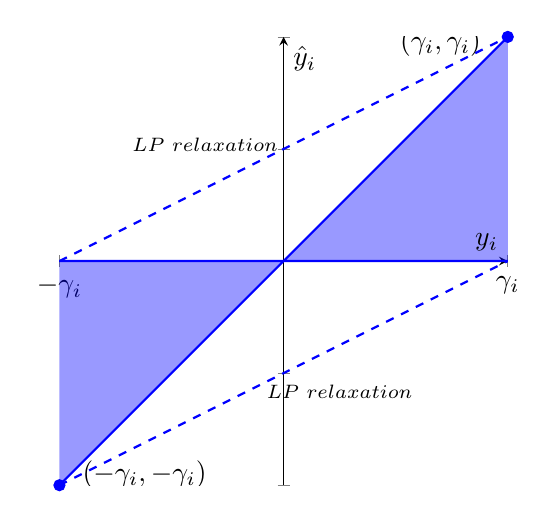
\begin{tikzpicture}
		\begin{axis}[
			xlabel={$y_i$},
			ylabel={$\hat{y}_i$},
			xmin=-2, xmax=2,
			ymin=-2, ymax=2,
			axis lines=center,
			samples=100, 
			unit vector ratio=1 1 1, scale=1, xtick   = {-2,2},
			xticklabels = {$-\gamma_i$,$\gamma_i$},
			yticklabels = {},
			]
			\addplot[blue, thick, fill=blue, fill opacity=0.4] {x} \closedcycle; 
			\addplot[blue, thick] {0}; 
			
			\addplot[only marks, mark=*, mark size=2pt, blue] coordinates {(-2,-2)};
			\node[label={above:$(-\gamma_i,-\gamma_i)$}] at (axis cs: -1.24, -2.2) {};
			
			\addplot[only marks, mark=*, mark size=2pt, blue] coordinates {(2,2)};
			\node[label={above:$(\gamma_i,\gamma_i)$}] at (axis cs: 1.4, 1.65) {};
			\addplot[dashed, thick, blue] coordinates {(-2,-2) (2,0)};
			\addplot[dashed, thick, blue] coordinates {(-2,0) (2,2)};
			\node[label={above:\scriptsize $\text{LP\ relaxation}$}] at (axis cs: -0.7, 0.8) {};
			\node[label={above:\scriptsize $\text{LP\ relaxation}$}] at (axis cs: 0.5, -1.4) {};
		\end{axis}
	\end{tikzpicture}
	\caption{Possible values of $\hat{y}_i$ depending on $y_i$ for the {\em 1b} model.}
	\label{fig.1v}
\end{figure}


  \begin{proposition}
	\label{prop5}
	Given $y_i \in [-\gamma_i,\gamma_i]$, 
	$\hat{y}_i$ is a solution of the MILP program :\begin{align*}
		\hat{y}_i &\leq a \gamma_i               &\quad \hat{y}_i &\geq y_i - a \gamma_i \\
		\hat{y}_i &\geq (a-1) \gamma_i           &\quad \hat{y}_i &\leq y_i + (1-a) \gamma_i
	\end{align*} where $a \in \{0,1\}$ is a binary variable.
\end{proposition}

\begin{proof}[Proof] First, we list the inequalities: \begin{align*}
		\hat{y}_i &\leq a \gamma_i               &\quad \hat{y}_i &\geq y_i - a \gamma_i \\
		\hat{y}_i &\geq (a-1) \gamma_i           &\quad \hat{y}_i &\leq y_i + (1-a) \gamma_i
	\end{align*}
	
	Similar to Proposition 4, we consider by cases.
	
	\textbf{$\mathbf{a = 0}$:} In this case, the inequalities become: \begin{align*}
		\hat{y}_i &\leq 0               &\quad \hat{y}_i &\geq y_i \\
		\hat{y}_i &\geq -\gamma_i           &\quad \hat{y}_i &\leq y_i + \gamma_i
	\end{align*} Now we can see, $y_i\leq 0$ (line 1) and $y_i\leq\hat{y}_i\leq 0 $. Line 2 is implied by other inequalities since \begin{align*}
	\hat{y}_i &\geq y_i \geq -\gamma_i           &\quad \hat{y}_i &\leq 0 \leq y_i + \gamma_i
	\end{align*}

	\textbf{$\mathbf{a = 1}$:} In this case, the inequalities become: \begin{align*}
		\hat{y}_i &\leq \gamma_i               &\quad \hat{y}_i &\geq y_i - \gamma_i \\
		\hat{y}_i &\geq 0           &\quad \hat{y}_i &\leq y_i 
	\end{align*} Now we can see, $y_i\geq 0$ (line 2) and $0\leq\hat{y}_i\leq y_i $. Line 1 is implied by other inequalities since \begin{align*}
	\hat{y}_i &\leq y_i\leq \gamma_i               &\quad \hat{y}_i &\geq 0 \geq y_i - \gamma_i 
	\end{align*}
		
Now we finish the proof. 
\end{proof}

\begin{figure*}[b!]
	\centering
	
\includegraphics[scale=0.75]{PIPE.pdf} 
	\vspace{-0.5cm}
	\caption{Training and bound computation on the pipe use case. 
		Two LAE-encoders are used, for the input (deformation) and for the output space (plastic strain). The surrogate is learned from reduced deformation input to reduced strain output.}
	\vspace{-0.2cm}
	\label{fig.PIPE}
\end{figure*}	



\section{Appendix for Section 6: {\em Diff} for robustness in regression tasks}


Our {\em Diff} model is not only accurate for classification. It can also provide upper bounds on the output of the DNN-regressor due to small perturbations of the input.
We consider here a pipe system and its DNN regressor from \cite{aiware},
that predicts the plastic strain in 3000 points of a mesh over a pipe given the deformation of each of these 3000 points.
Compared to the classification tasks where the DNN is learned in a standard way and LAE is later applied to reduce the input dimension without compromising the accuracy, the DNN regressor has been learned on the reduced LAE feature space directly, for both the high-dimensional input and the high-dimensional output (3000 dimensions each).







Figure \ref{fig.PIPE} describes the pipeline used to learn the DNN regressor for the pipe system. The DNN that has been learned has 2 fully connected layers, 50 neurons each, learned as a surrogate model, with 10 reduced inputs and 26 reduced outputs.

In terms of perturbation, we consider a conjunction of $L_1 \leq 3.9$ and $L_\infty \leq .02$ perturbations, physically pertinent dimensions, and maximize the sum of the difference in output of 10 selected points in the mesh between the input and its deformation.





\begin{table}[h!]
	\centering
	\begin{tabular}{|c | c c c c c|} 
		\hline
		Pipe & Timeout & ITNE & {\em Diff} & {\em 2$b+$1} & {\em 1$b$}
		\\\hline 
		& 1000s & 0.045 & 0.042 & 0.041 & {\bf 0.036}
		\\
		Surrogate  & 14400s & 0.042 & 0.036 & {\bf 0.035} & 0.036
		\\
		LB = $.025$  & 72000s & 0.042 & 0.034 & {\bf 0.033} & 0.036
		\\\hline
	\end{tabular}
	\caption{Comparison of upper bound (lower is better $\downarrow$) between {\em Diff}, {\em 2$b+$1}, {\em 1$b$} with ITNE on the pipe system with timeouts of 1000s, 14400s and 72000s.}
	%L1 corresponds to $3.9$ or $4$, and results should be the sum of 10 pixels, so around 10 times higher values.}
\label{table.pipe}
\end{table}




For the pipe system, we compare in Table \ref{table.pipe} the different models ITNE, {\em Diff}, {\em $2b+1$,$1b$} to produce bounds on the sum of the difference of strain over 10 specific points of the mesh, for a physically relevant perturbation of the deformation. 
The bounds we found are quite accurate, with a best bound of $.033$ obtained by the {\em $2b+1$} model, slightly better than the bound $.034$ found within the same time by the {\em Diff} model, and better than the bound found $.036$ by the {\em "$1b$"} model, although this bound has been found 70 times faster due to the simpler model ({\em 1}$b$ converges after 1000s). ITNE is significantly worse than even the {\em "$1b$"} with 1000s of timeout, at $.042$ despite a very long timeout. The certified lower bound is not too far, at $.025$.

We did check that this worst-case found, displayed in Fig. \ref{fig5} and which is not too far from the actual worst case that is known to be $<.033$, is coherent with the physical finite element model the DNN surrogate has been learned from. Hence, this brittleness of the surrogate is {\em not} a hallucination due to the learning process, but rather correctly reflects the physical system.


\begin{figure*}[b!]
\centering
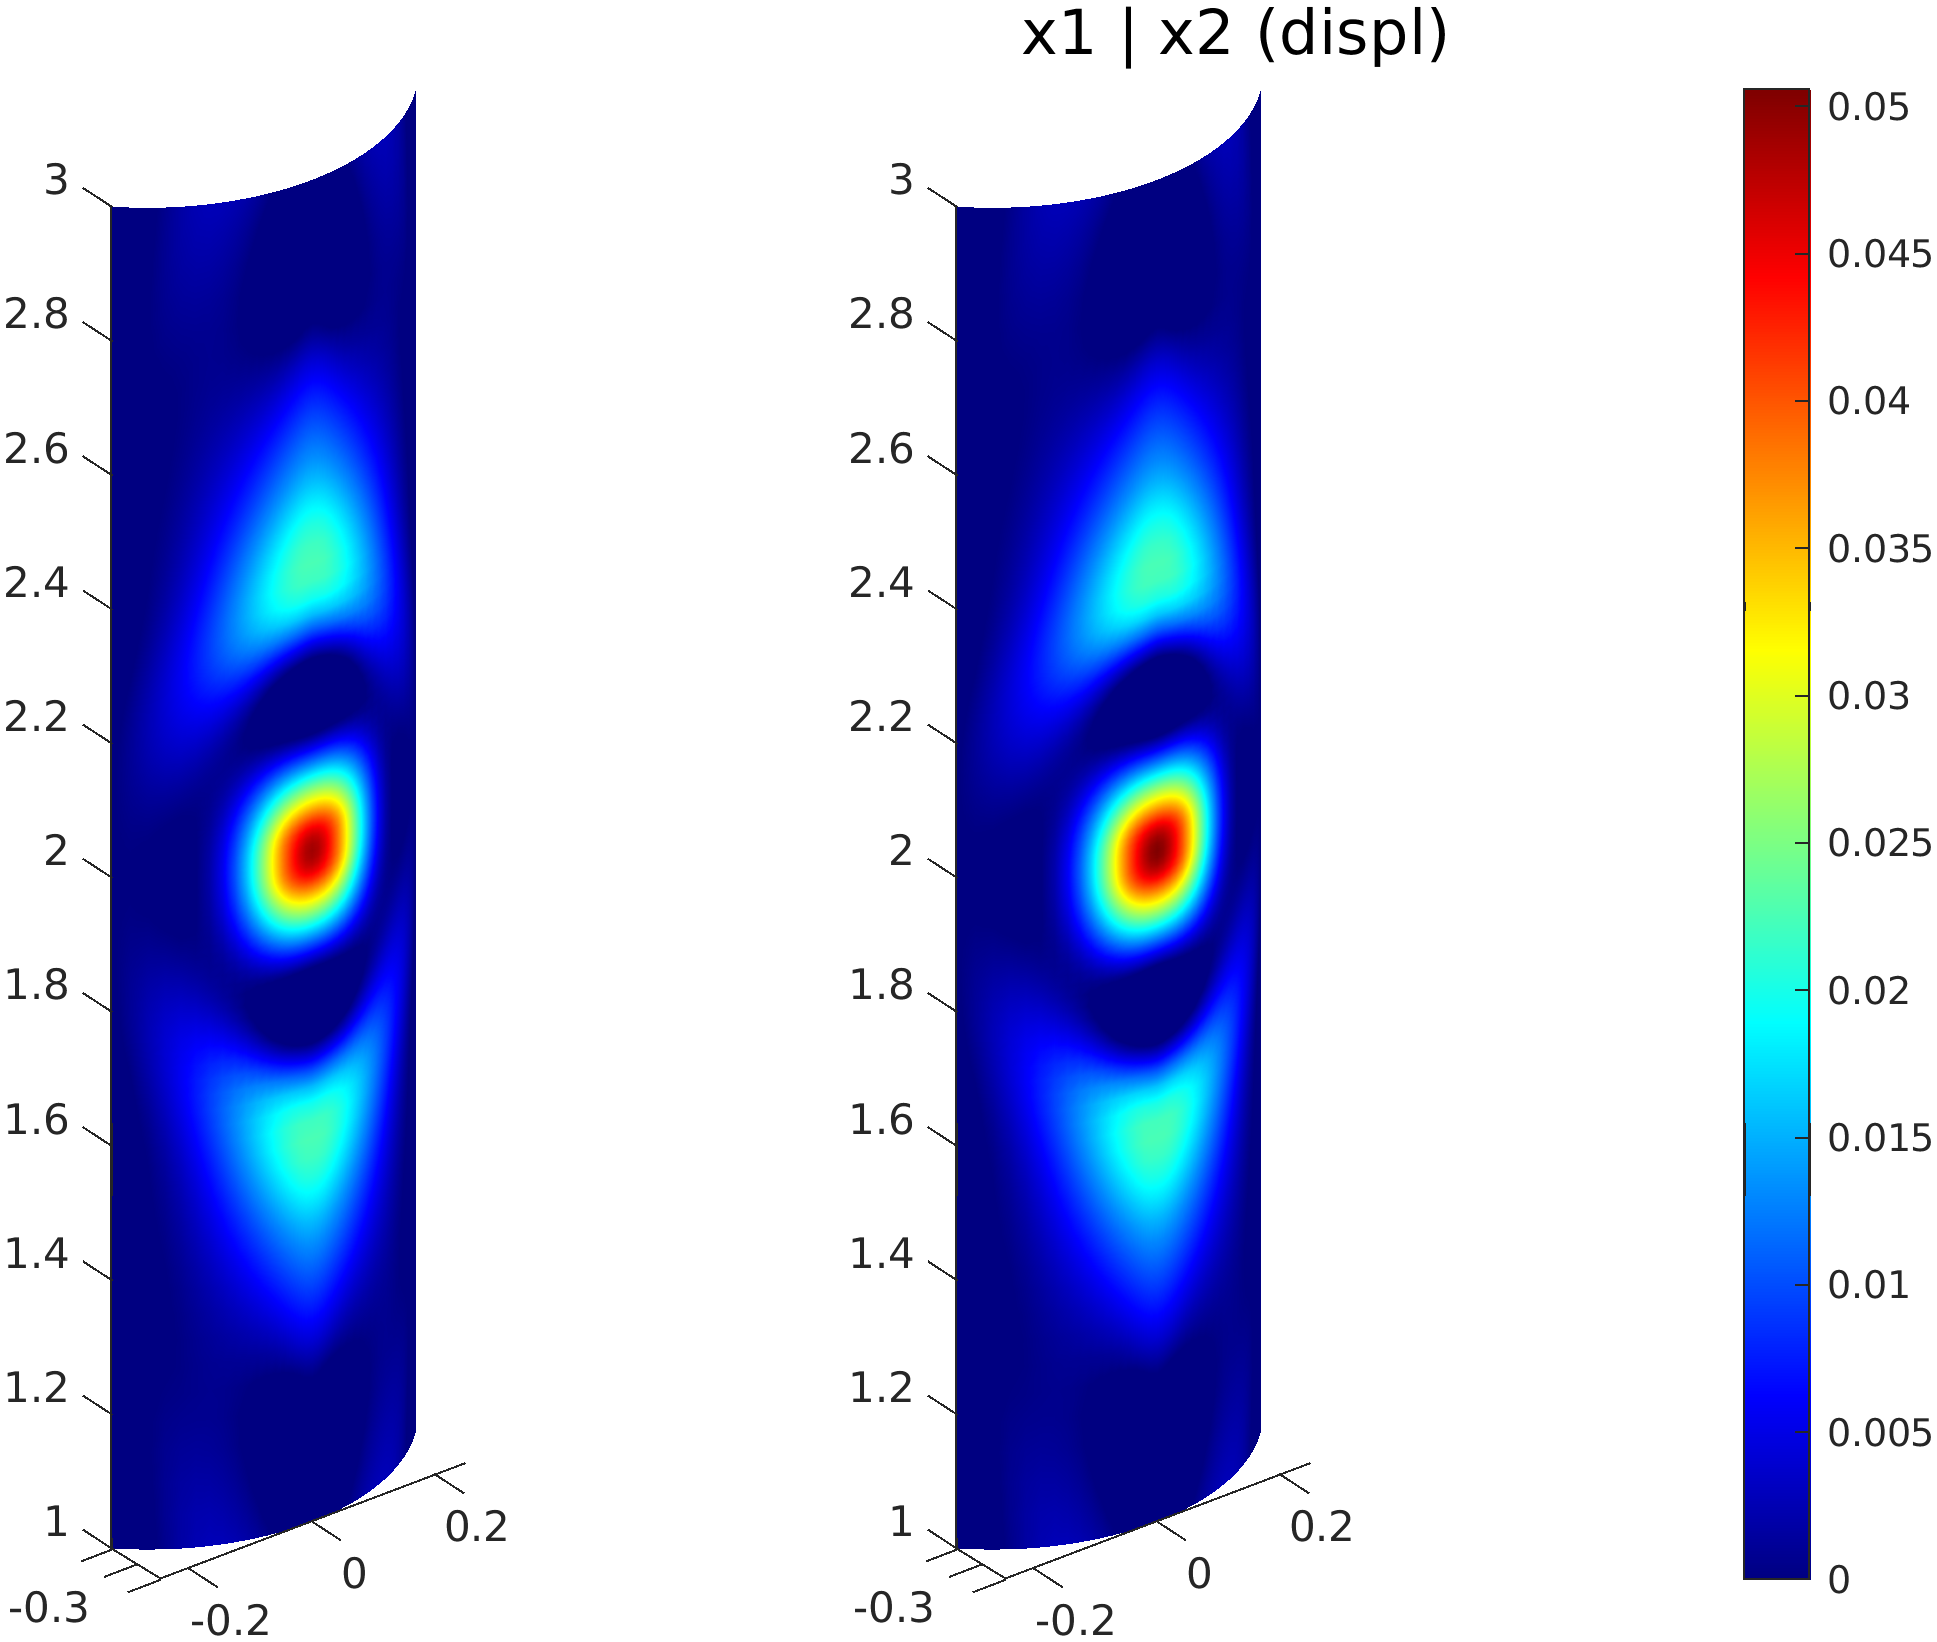
\includegraphics[scale=0.36]{deform.png} \hspace{0.1cm}
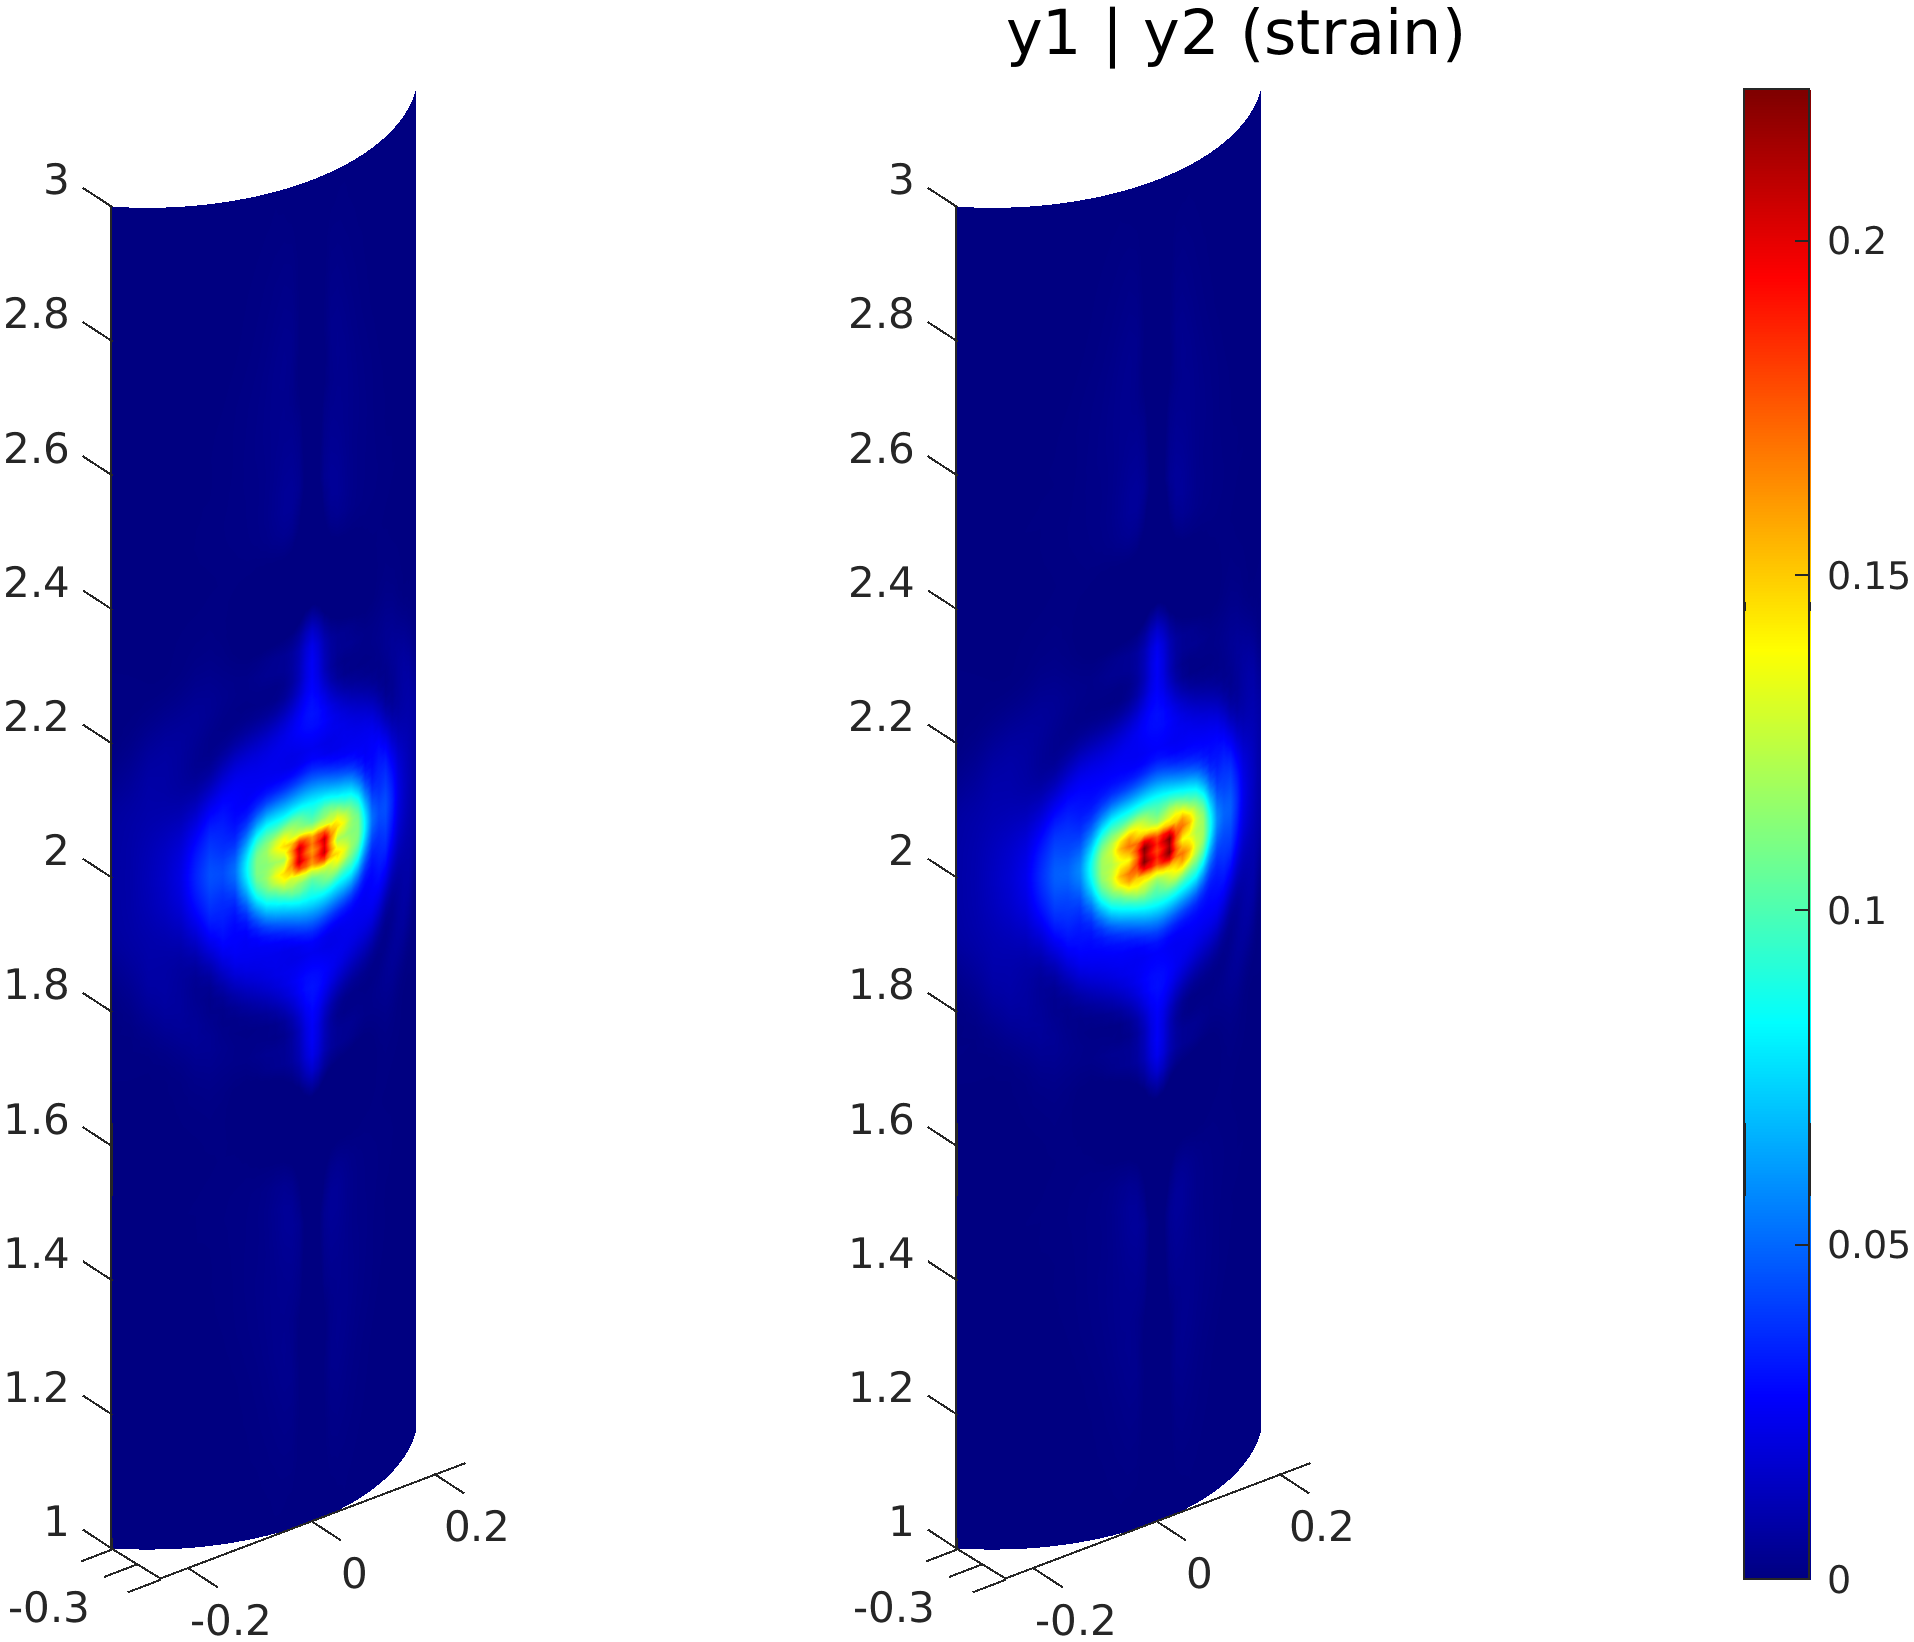
\includegraphics[scale=0.36]{strain.png}
\caption{2 slightly different deformations and their associated quite different strain as obtained by the {\em Diff} model with $200 $ binary variables.}
\label{fig5}
\end{figure*}	


